\documentclass[journal]{IEEEtran}
\usepackage{amsmath,amssymb,amsfonts}
\usepackage{tabularx}
\usepackage[utf8]{inputenc} % allow utf-8 input
\usepackage[T1]{fontenc}    % use 8-bit T1 fonts
\usepackage{url}            % simple URL typesetting
\usepackage{booktabs}       % professional-quality tables
\usepackage{amsfonts}       % blackboard math symbols
\usepackage{nicefrac}       % compact symbols for 1/2, etc.
\usepackage{microtype}      % microtypography
\usepackage{graphicx}
\usepackage{float}
\restylefloat{table}
\usepackage{hyperref}
\usepackage{multicol}
\usepackage{caption}
\usepackage{subcaption}
\usepackage{amsmath}
\usepackage{algorithm}
\usepackage{algpseudocode}
\usepackage{tikz}
\usetikzlibrary{trees}
\usepackage{listings}
\usepackage{array}
\usepackage{colortbl,hhline}
\usepackage{color}
\usepackage{xcolor}

\DeclareMathOperator*{\argmax}{arg\,max}  % in your preamble
\DeclareMathOperator*{\argmin}{arg\,min}  % in your preamble

\usepackage{textcomp}

%\usepackage[retainorgcmds]{IEEEtrantools}
%\usepackage{bibentry}
\usepackage{xcolor,soul,framed} %,caption

\usepackage[noadjust]{cite}
%\usepackage{biblatex}
%\bibliographystyle{plain}

\usepackage[font=scriptsize]{caption}
\captionsetup[figure]{font=scriptsize}
%=== TITLE & AUTHORS ====================================================================
\begin{document}
\bstctlcite{IEEEexample:BSTcontrol}
    \title{test}
\title{Coaching with PID Controllers: A Novel Approach for Merging Classic Control with Reinforcement Learning}

\author{ Zongqiang Pang, Liping Bai \thanks{Nanjing Unversity of Posts and Telecommunications, College of Automation \& College of Artificial Intelligence, Nanjing, Jiangsu,210000 China email:zqpang@njupt.edu.cn}}
% ====================================================================
\maketitle
% === ABSTRACT ====================================================================
% =================================================================================
\begin{abstract}
In this paper, we propose a PID controller based coaching scheme in order to expidite data collection on critical states and accelerate reinforcement learning (RL). In previous attempts for fusing classical control and RL, training accelerations are brought about with the cost of implicit caps on what is attainable by the RL agents, and high quality controllers are essential. We ask if it possible to accelerate RL with even a basic hand-tuned PID controller and we draw inspiration from the relationship between atheletes and their coaches. World class atheletes are by definition the top of their field, yet training with coaches who are less capable than them is still an integral part of their skills acquisition process. The job of a coach is not to function as a template to be imitated, but rather to provide conditions for the atheletes to collect critical experiences and that is what we seek to replicate in our approach. Experiments are conducted in Mujoco locomotion environments and we conclude from the data that when the coaching structure between PID controller and RL agents is set at its goldilocks spot, agents training can be accelerated, in some cases significantly, yielding uncompromised training results in the mean time. This is an important proof of concept that controller based coaching can be a novel and effective paradigm for merging classical control with learning and warrants further investigations along this direction. All the code and data can be found at: \href{https://github.com/BaiLiping/Coaching}{github.com/BaiLiping/Coaching}
\end{abstract}
% === KEYWORDS ====================================================================
% =================================================================================
\begin{IEEEkeywords}
Reinforcement Learning, Control, L4DC
\end{IEEEkeywords}
\IEEEpeerreviewmaketitle
% === I. Paper =============================================================
% =================================================================================
\section{Introduction}
\IEEEPARstart{R}{einforcement} Learning (RL) is a cyle between interaction with the environment and refinement of the understanding of that environment. RL agents methodically extracting information from experiences, gradually bounding system models, policy distributions or cost-to-go approximations to maximize the expected rewards along a trajectory. While the field of RL routinely generate jaw-dropping results \cite{Mnih2013PlayingAW}\cite{Hausknecht2015DeepRQ}\cite{Andrychowicz2020LearningDI}\cite{Kalashnikov2018QTOptSD}\cite{Lee2020LearningQL}, there are aspects of its methodology that are inherently inefficient. The focus of current researches is to re-formulate RL to be more effective.

There are four angles of attack in order to address the inefficiencies. First, researchers who are well versed in statistics and information theories approach the problem by devising ever more sophisticated statistical processes to push the budgeted data collection and information extraction to its limit.\cite{Ho2016GenerativeAI}\cite{Finn2016UnsupervisedLF}\cite{Pathak2017CuriosityDrivenEB}\cite{Burda2019LargeScaleSO}\cite{Finn2017ModelAgnosticMF}\cite{Mishra2018ASN}\cite{Nachum2018DataEfficientHR}\cite{Vezhnevets2017FeUdalNF}\cite{Blundell2015WeightUI}\cite{Gal2017ConcreteD}\cite{Dasgupta2019CausalRF}\cite{Zhang2020DesigningOD} Second, control theoriests who are capable of wielding optimization techniques and mathematical formalism provide a systematic perspective to RL and invent the much needed analytical tools.\cite{Han2020ActorCriticRL}\cite{Weinan2017APO}\cite{Dupont2019AugmentedNO}\cite{Betancourt2018OnSO}\cite{Nachum2020ReinforcementLV}\cite{Luo2019ADR}\cite{Wu2020DataDrivenDL}\cite{Shi2019NeuralLS}Third, CHANGE THIS TO SYSTEM INDENTIFICATION. \cite{Hewing2020LearningBasedMP}\cite{Mohan2020EmbeddingHP}\cite{Lusch2018DeepLF}\cite{Bai2019DeepEM}\cite{BelbutePeres2020CombiningDP} Fourth, imitation learning, reverse reinforcement learning, and human-in-the-loop teaching aim at preemptively limitsing exploration to the pertinent states and providing guidance to the data collection process. \cite{Knox2009InteractivelySA}\cite{Knox2010CombiningMF}\cite{Peng2018DeepMimicED}\cite{Peng2020LearningAR}\cite{Paine2018OneShotHI}

In this paper, we propose an additional angle of attack: classical controllers based coaching. We are not the first group to realize that classical controllers can be used to guide RL agents and accelerate training. \cite{Xie2018LearningWT}\cite{Carlucho2017IncrementalQS}\cite{Pavse2020RIDMRI}. Yet all the previous works demand high quality controllers to begin with and the improvements brought about by the RL agents are merely icing on the cake. In addition, the controllers inadvertently impose limits on what can be achieved by the RL agents, if a bad controller is chosen, then the RL training process would be hindered rather than expedited. We ask the question, is there a way to take advantage of hand-tuned PID controllers, which might not be high-quality but still captures some of our understanding of the system, in the RL training process? This inquiry lead us to the relationship between atheletes and their coaches.

Professional athletes don't get where they are via trial-and-error. Their skillsets are forged through coaching. Have you ever wondered why top atheletes who represent the best in that sport still need coaching from people who are less capable? The objective of a coach is to facilitate data collection on critical states, therefore the capacity of the coach per se is not essential for training purposes. This provide us with empirical evidence that training acceleration can be achieved with properly constructed coaching scheme, and the demand on controller quality should not be strigent. 

In this paper, we hand-tune the PID controllers as the 'coaches'. The performance of the PID controllers is miserable comapare to the respective RL agent as shown by Figure \ref{fig:pid}. Yet, even with such bad controllers, when structured properly, training acceleration is still observed, as shown by Figure \ref{fig:comparison}. The detailed of our implementation and caveats would be detailed in subsequent sections.

\begin{figure}
\centering
\begin{subfigure}{0.25\textwidth}
  \centering
  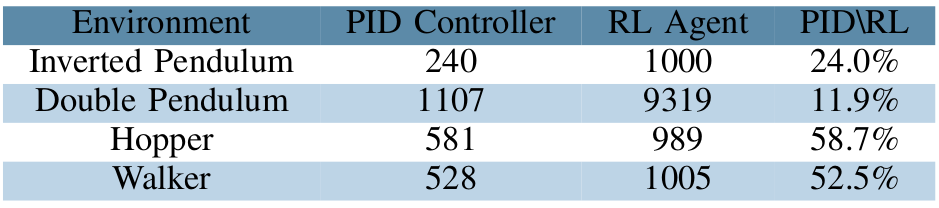
\includegraphics[width=\linewidth]{PIDvsRL.png}
  \caption{Performance Comparison. Hand-Tuned PID controllers perform miserably compare to the perepective RL agent.}
  \label{fig:pid}
\end{subfigure}%
\begin{subfigure}{.25\textwidth}
  \centering
  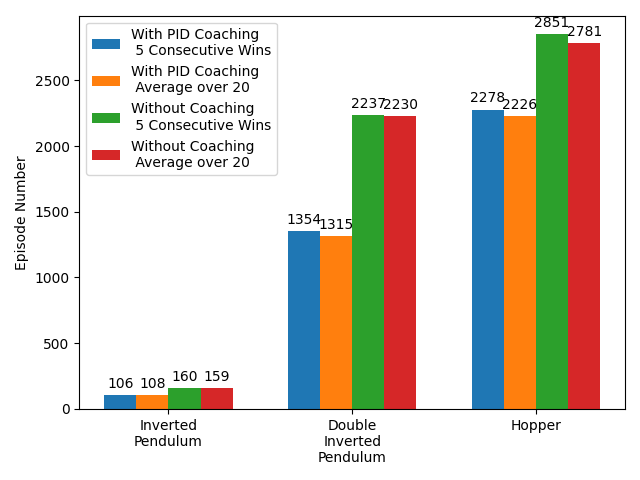
\includegraphics[width=\linewidth]{compare.png}
  \caption{Even though the PID controllers are less capable than the eventual RL agent. During the training phase, it is still helpful and can accelerate the RL agent training, as indicated by the number of episodes training required to reach a predetermined target score.}
  \label{fig:comparison}
\end{subfigure}
\end{figure}


\begin{table}
\footnotesize
\caption{PID Controller Vs Agent Score}
\label{score}
\centering
\begin{tabular}{ |c|c|c|c| }
\hline
\cellcolor[HTML]{6195C9}Environment & \cellcolor[HTML]{6195C9}  PID Controller &\cellcolor[HTML]{6195C9}RL Agent &\cellcolor[HTML]{6195C9}PID\textbackslash RL \\
\hhline~
Inverted Pendulum &  264 & 1001& \cellcolor{lightgray}26.4\%\\
\hhline~
Double Pendulum &  358 & 9319&3.8\%\\
\hline
Hopper &  303 & 989&30.6\%\\
\hline
Walker &  332 & 1009&32.9\%\\
\hline
\end{tabular}
\end{table}


\begin{table}
\scriptsize
%\renewcommand{\arraystretch}{1.3}
%\newcolumntype{x}[1]{>{\centering\arraybackslash\hspace{0pt}}p{#1}}

\caption{Comparison Between Agents Trained With and Without PID Controller Coaching}
\label{table_example}
\centering
\begin{tabular}{ |c|c||c|c|c|c| }
\hline
Environment & Target & Measure  &  With PID  & Without  & Percentage\\
   Name     & Score  &              & Coaching  & Coaching  & Increase \\
\hline
\hline


Inverted & 800& 5 Wins & 106 & 160& 23\% \\
Pendulum & &Average  & 108 &  159& 13\%\\
\hline
Double & 800& 5 Wins & 106 & 160\\
Pendulum & &Average & 108 &  159\\
\hline
Hopper & 800& 5 Wins & 106 & 160\\
       & &Average  & 108 &  159\\
\hline
Walker & 800& 5 Wins & 106 & 160\\
       & &Average  & 108 &  159\\
\hline

\end{tabular}
\end{table}




In section II we provide the basic understanding of reinforcement learning as seen from control perspective. In section III, we present the results of all our experiments. While the experiments are conducted in Mujoco simulated environment, we consciously designed things in a way such that it can be conveniently implemented in the physical world as well. In the final section, we conclude what we have learned from our experiments and layout directions for further research.



\section{From Optimization To Learning}

Reinforcement Learning is not a new subject, control researchers probably know it by the name Approximate Dynamic Programming (ADP) or Neuro Dynamic Programming (NDP). When the first batch of reasonable RL results was introduced, it was met with coldness by people in control. The preface of Bertseka's book Neuro Dynamic Programming provides a good sample of how RL was perceived by the control community back in 1996: "...These methods (Reinforcement Learning) were aiming to provide effective suboptimal solutions to complex problems of planning and sequential decision making under uncertainty, that for a long time were thought to be intractable. Our first impression was that the new methods were ambitious, overly optimistic, and lacked a firm foundation. Three years later, after a lot of study, analysis, and experimentation, we believe that our initial impressions were largely correct." \cite{Bertsekas1996NeuroDynamicP}

Today, the theoretical foundation of RL is as bleak as it was in 1996, but its deficiencies can be easily papered over with the advant of Neural Networks and ever more impressive computational capacities. Before 2010, the predominant function approximators are handcrafted kernels, where feature spaces transform nonlinear functions into linear space. Today, the default function approximator is Deep Neural Network and its variants. In the computation front, Graphic Process Unit (GPU) based parallelization is accessible to anyone who is proficient with C/C++\cite{Nickolls2008ScalablePP}, and software packages such as PyTorch\cite{Paszke2017AutomaticDI} and Tensorflow\cite{Abadi2016TensorFlowAS} made this task even more trivial.

In order to better introduce RL to control researchers, we built on Benjamin Recht's presentation\cite{Recht2018ATO}, framed RL in the language of optimization. Reinforcement Learning is an umbrella term, which encompasses distinctive genres of learning. Learning in the context of RL means updating parameters of the function approximators. Categorically speaking, there are three avenues where learning finds its way into optimization as shown in Figure\ref{fig:1}. 
\begin{figure}
    \centering
    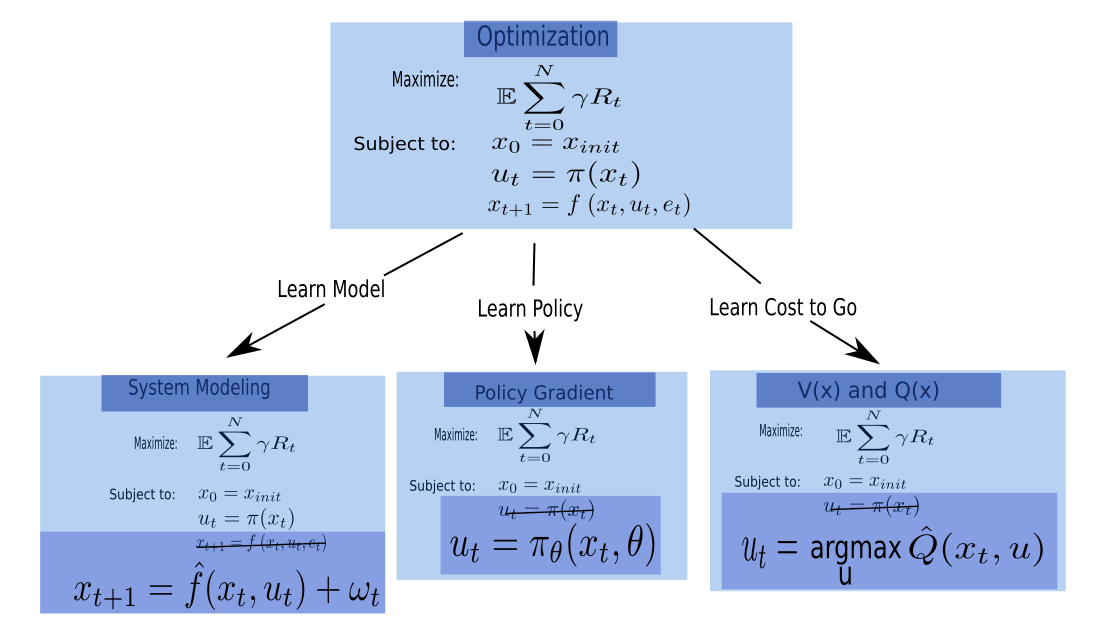
\includegraphics[width=0.5\textwidth]{Control.png}
    \caption{From Optimization to Learning}
    \label{fig:1}
\end{figure}

Model-Based or Model-Free learning refers to whether or not learning is used to approximate the system dynamics function. If there is an explicit action policy, it is called on-policy learning. Otherwise, the optimal action would be implicitly captured by the Q value function and that would be called off-policy learning instead. Importance sampling allows "limited off-policy learning" capacity, which allows data reuse in a trusted region. Online learning means interleaving data collection and iterative network parameters update. Offline learning means the data is collected in bulk first and then the network parameters are set with regression computation. Batch learning, as the name suggested, is in between online and offline learning. An agent would first generate data that fill its batch memory and then sample from the batch memories for iterative parameter update. New data would be generated with the updated parameters to replace older data in the memory. This taxonomy is somewhat outdated now. When Richard Sutton wrote his book, the algorisms he had in mind fall nicely into various categories. Today, however, the popular algorisms would combine more than one route to derive superior performance, and can't be pigeonholed.

We will not go into the details of various RL algorithms and the zoo or acronyms that come with it, as that is beyond the scope of this paper. PPO agents were chosen for all our experiments because the learning curves generated by PPO agents are smoother compare to other agents. The goal of our paper is to indicate the proposed active boundary method works, which is easier to be shown with smoother curves. However, we would like to point out two crucial concepts that undergird the feasibility of reinforcement learning.

\subsection{Bellman Update}

Reasoning backward or Dynamic Programming forms the basis of reinforcement learning. If we know the desired final state and system dynamics then we can simply compute backward on the penultimate step. Set the penultimate step as the final step, then repeat the process until the action strategy for the initial state is obtained. This approach, Bellman Update, would work if two prerequisites are met: first, the system dynamics function is known; second, the dimensions of observation space and action space are small. Neither would be true for the problems we encounter in the real world.

When the dynamics are unknown yet the dimensions of the problem are manageable, the cost-to-go lookup table can be constructed with sampling methods. As mentioned earlier, the way that the lookup table is updated with the sample can be categorized by the horizon of the data collection. If the lookup table is updated with data collected from an entire episode, it is called the Monto Carlo method. If the lookup table is updated every step, it is called Temporal Difference method, and there are various methods in between these two extremes. When the dimensions of the problem are large in addition to unknown dynamics, function approximators are used for the system model, the policy function, or the cost-to-go function. 

Immediately, control researchers can spot the deficiency with the latter case. For backward reasoning to work properly, the notion of optimality has to be satisfied either through known dynamics function or robust sampling methods, yet when the dynamics are unknown and the dimensions large, the notion of optimality can no longer be guaranteed through sampling. This is where the expertise of statisticians and information theoriests comes in and the research topic of exploration-exploitation trade-off.

\subsection{Bootstrap}

Another fundamental concept for RL is convergence through bootstrap. Instead of asymptotically approaching a known target function, bootstrap methods approach an assumed target first and then update the target assumption based on collected data. This process is illustrated by Figure\ref{fig:bootstrap}. Intuitively, when estimation functions are evaluated with assumption instead of the true value, things could just run around in circles and never converge. That is indeed the case before the introduction of DQN\cite{Osband2016DeepEV}. As a matter of fact. the stability and convergence achieved in that paper are more of a reflection on the techniques and know-how of the DeepMind team. Initially, those results can not be easily replicated by other labs. Even today, instability in RL is still a major research focus. 

\begin{figure}
\centering
\begin{subfigure}{0.25\textwidth}
  \centering
  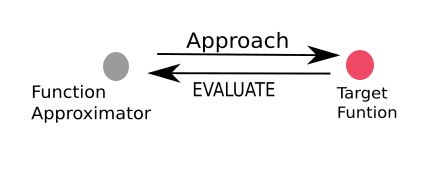
\includegraphics[width=\linewidth]{onego.png}
  \caption{With Known Evaluation Function}
\end{subfigure}%
\begin{subfigure}{.25\textwidth}
  \centering
  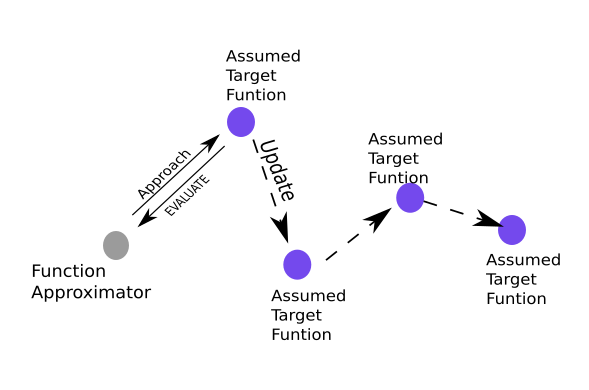
\includegraphics[width=\linewidth]{bootstrap.png}
  \caption{Bootstrap}
\end{subfigure}
\caption{Convergence through Bootstrap}
\label{fig:bootstrap}
\end{figure}



\section{Experimental Setup}

Mujoco physics engine does provide the system models for the simulation, therefore it is possible to compute for more sophiscated controllers.


We implemented our active boundary experiments in OpenAI Gym\cite{Brockman2016OpenAIG} as a proof of concept. We are cognizant of the fact that eventually, things should apply to a real-world scenario. Therefore, we designed the active boundary in a manner such that it can be swiftly adapted to physical implementation. Agents are implemented with tensorforce\cite{tensorforce}. We sorted out the observation space and action space for each environment and recorded them in the code of each experiment.

As we suggested in the previous section when agents reach the critical state, "correct actions" would be applied by the active boundary to the agent, hence the name "active". Much like a coach would guide athletes through the most crucial step of the training. We also designed a penalty term associated with active boundary to discourage its use. If the agent act flawlessly at the critical state, no penalty would be applied. On the other hand, if the agent requires active boundary intervention, a penalty term would be registered. 

The positions and penalty terms are set in an ad hoc fashion in our experiments. At this point, we do not have an analytical frame that can guide us in making such decisions. We choose three positions for the boundary during each experiment and 4-6 penalty terms ranging from 0 upwards. The rule of thumb we used for the penalty is that the punishment score should be comparable to the reward.

Our experiments are conducted over the following environments: CartPole, with discrete action space; Inverted Pendulum, with continuous action space; Inverted Double Pendulum; Hopper; Walker2D. We did not implement our approach to more sophisticated environments such as HalfCheetah, Humanoid, and HumanroidStandup due to hardware constraints. Yet we feel that for the data we collected, our approach has shown conclusive results. The following are our experiment setup and results.

The dashed black lines are the training results of agents with normal training, which functions as the control group and the benchmark. The colored lines are the results of agents trained with varying penalty terms. The average evaluation scores of the agents are presented at the upper left corner of the graph.

\subsection{Inveretd Pendulum}
CartPole's Observation Space is the vector: [Cart Position, Cart Velocity, Pole Angle, Pole Angular Velocity]. The discrete action space for cartpole is: [Push Cart to the left, Push cart to the right]. The continuous action space for Inverted Pendulum is an action ranging from -1 to 1, where -1 means the actuator moves the cart to the left with maximum power and 1 means the actuator moves the cart to the right with maximum power. The maximum episode step number for cartpole and inverted pendulum are 500 steps and 300 steps respectively. The terminal state for cartpole is angle of absolute value greater than 24 degrees. The terminal state for the inverted pendulum is an angle of absolute value greater than 0.2 radius. The reward for cartpole and inverted pendulum are both 1 for each step and 0 for the terminal step. 

The active boundary is implemented as a ring anchored on the cart, at the height of the middle of the pole. Touch sensors would be installed in order to detect contact between the pole and the ring. We propose three sets of rings each allows a maximum angle of 0.5, 0.7, and 0.9 of the terminal state angle in the cartpole environment and 0.1, 0.4, 0.5 radii in the inverted pendulum environment, as shown by Figure \ref{fig:cartpolePB}. 

When contact between the pole and the active boundary is detected by the sensor, the cart would be pushed towards the appropriate direction depending on the sign of the angle. This step can be easily programmed by a microcontroller in physical implementation, and for implementation in simulation, it is just a matter of specifying a premeditated action. For detailed code, please refer to the code depository. Note that should the boundary is set without touch sensors and the corresponding actions, it would just be a passive boundary instead of an active one. 

A penalty term, which is chosen from vector [0,-5,-7,-10,-12,-15], would incur every time the pole contacts the active boundary. Our experiment result on cartpole are shown by Figure \ref{fig:CartPole}. The experiment result on inverted pendulum is shown by figure \ref{fig:InvertedPendulum}. As the data suggest, when the boundary is set too restrictively, it severely hinders the training. The best results is seen when the boundary is set at 10.8 degrees. After the agents are done training, we evaluate their performance in normal environments, the average evaluation scores are presented at the upper left part of the graphs. Our data suggest that during the evaluation, agents with accelerated training perform comparably to the agents with normal training.
\begin{figure}
     \centering
      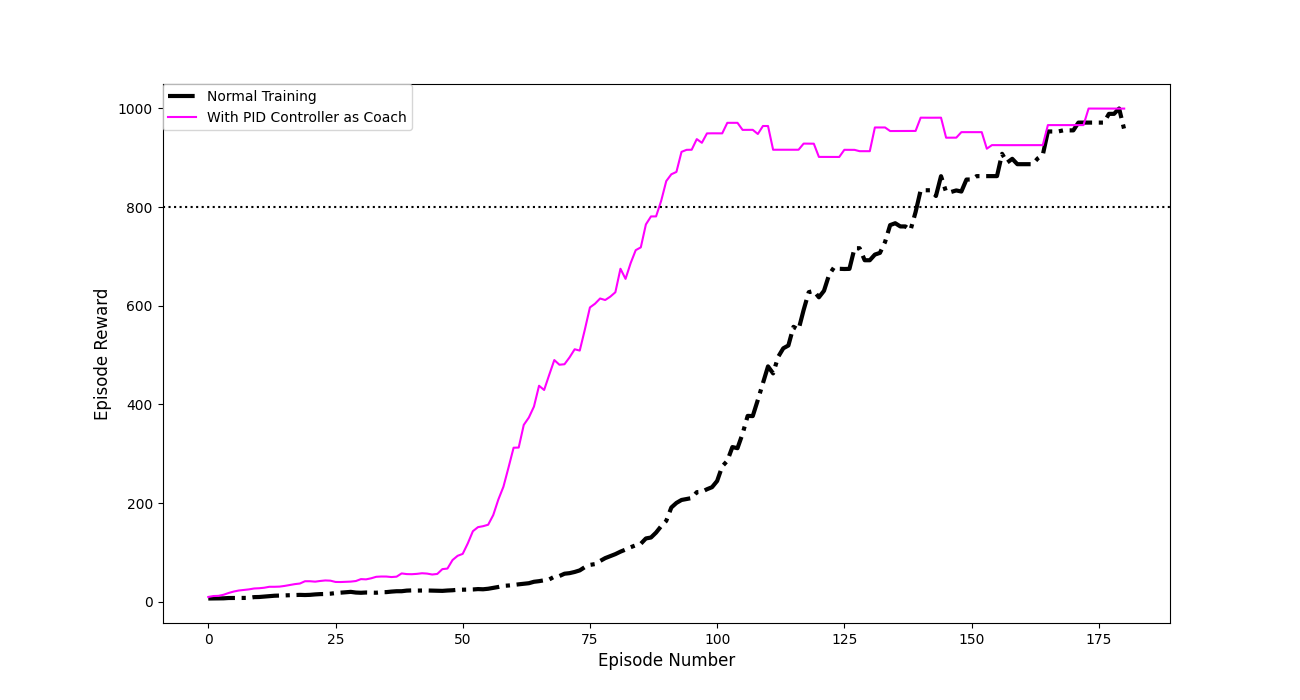
\includegraphics[width=0.5\textwidth]{ip.png}
      \caption{Inverted Pendulum Coaching Result. Benchmarked against training without coaching, indicated by the black dotted line.}
      \label{fig:ip}
\end{figure}

\subsection{Inverted Double Pendulum}
The inveretd double pendulum has observation space of the following: [x position of the cart, sin($\theta_1$), sin($\theta_2$),cos($\theta_1$),cos($\theta_2$),velocity of x, angular velocity of $\theta_1$, angular velocity of $\theta_2$, constraint force on x, constraint force on $\theta_1$, constraint force on $\theta_2$]. $\theta_1$ and $\theta_2$ are the angles of the upper and lower pole perspectively.

The action space for Inverted Double Pendulum is an action ranging from -1 to 1, where -1 means the actuator moves the cart to the left with maximum power and 1 means the actuator moves the cart to the right with maximum power.

The Terminal state of double inveretd pendulum is when the y postion of the upper pole, which can not be observed by the agent, falls below 1.

We design the active boundary to be located at the same height as does the joint between the upper and the lower pole, as indicated by Figure \ref{fig:doublePB}. The boundary allows the joint to flex for 0.4, 0.5 and 0.6 radii respectively, each with the penalty parameters of a choice between 0,-3,-4,-5,-6,-7. When the joint extends to touch the active boundary, an action of -1 or 1 would be automatically applied to rectify the situation, depending on the sigh of the angles.


Our experiment result is shown by Figure \ref{fig:Double Pendulum}. The conclusion is similar to that of cartpole and inverted pendulum results. When the active boundary is set at 0.4 radii, it hinders learning rather than facilitate it. When the boundary is set at 0.5 radii with a penalty parameter of -7, we see the most drastic acceleration of agent training. However, when the boundary is set at 0.6 radii, it seems to have given the agent too much flexibility since the result suggests that the acceleration is not as profound compare to that of the boundary set at 0.5.

\begin{figure}
     \centering
      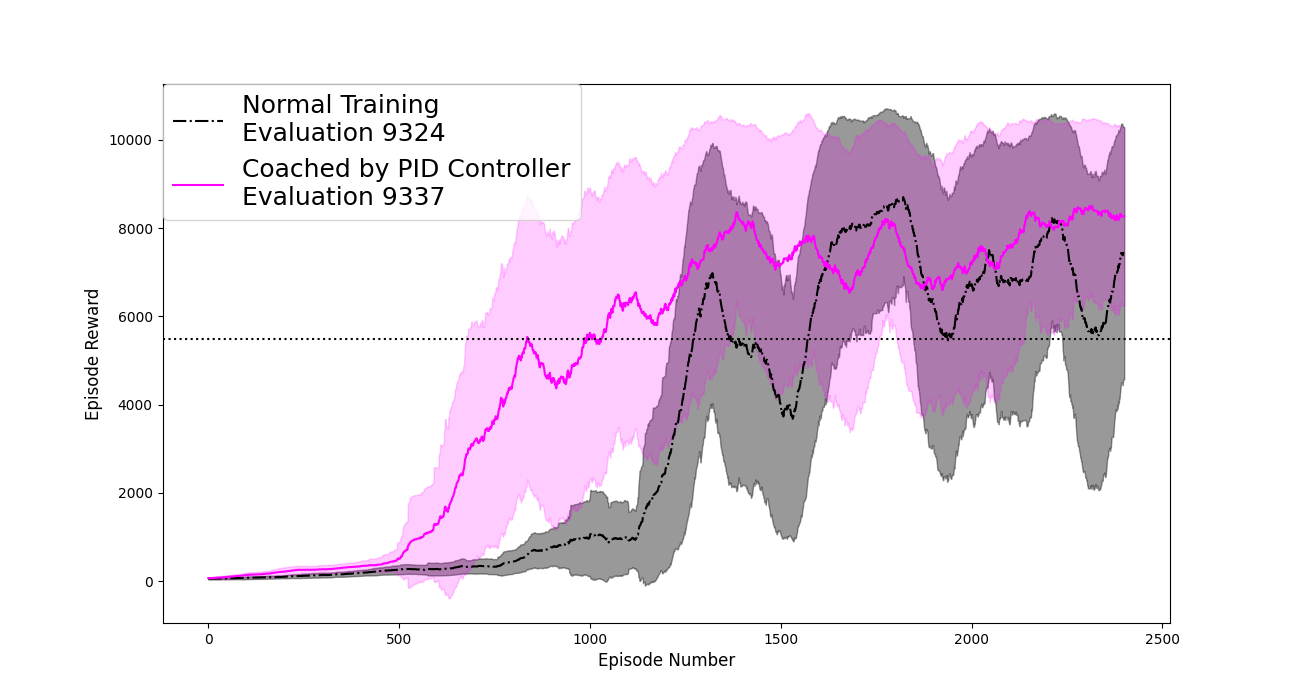
\includegraphics[width=0.5\textwidth]{double.png}
      \caption{Double Inverted Pendulum Coaching Result. Benchmarked against training without coaching, indicated by the black dotted line.}
      \label{fig:double}
\end{figure}

\subsection{Hopper}
The observation space of hopper is the following vector: [z position, y position, thigh joint angle, leg joint angle, foot joint angle, velocity at x-axis, velocity at z-axis, velocity at y-axis, angular velocity of thigh joint, angular velocity of leg joint, angular velocity of foot joint].

The action space of hopper are three continuous action choices for three actuators [thigh actuator, leg actuator, foot actuator]. The range of for actuators are -1, which means apply force towards the negative direction with maximum power, and 1 which means apply force towards the positive direction with maximum power.

The terminal states for hopper are when the absolute y position is greater than 0.2.

There are more than one ways to implement active boundary in hopper environment. Because we want things to be applicable in real-world scenarios, we chose the implementation with the easiest setup. In our experiment, the active boundary is defined with the y-position at 0.05, 0.1 and 0.15, each with the penalty parameters that is chosen from 0,-3,-5,-7,-10 as shown by Figure \ref{fig:hopperPB} When the agent touches the active boundary, we gently guide it slightly towards the center line, and the velocities terms are all set to zero. We seek to mimic how a coach would guide an athlete towards the desired trajectory during training. When the athlete is about to deviate off-course, the coach would take over and apply the appropriate force to slightly reset the trajectory. This can be implemented with an automatic harness in a physical experiment.

Our experiment result is shown by Figure \ref{fig:Hopper}. Similar to the conclusion drawn with previous data, when the active boundary is set too narrowly at 0.05 y position, it restricts the agent and almost completely halts the agent training. The best training acceleration is observed when the boundary is set at 0.15 y position.

\begin{figure}
     \centering
      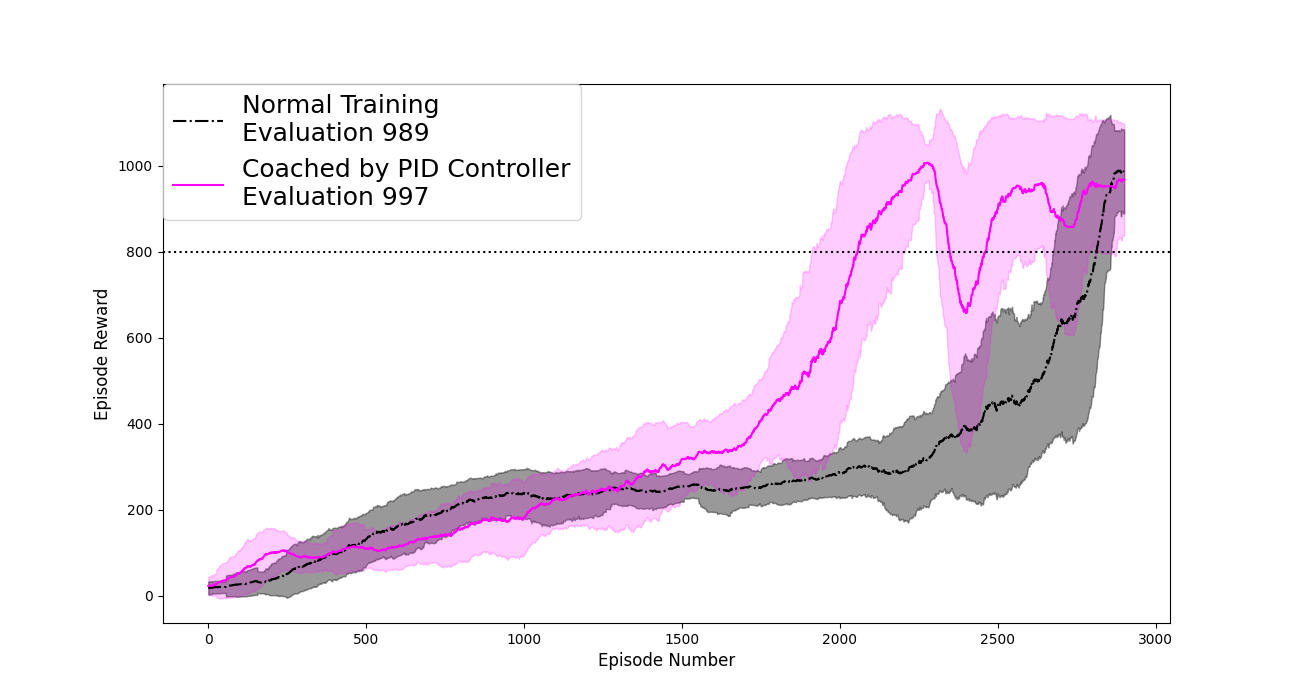
\includegraphics[width=0.5\textwidth]{hopper.png}
      \caption{Hopper Coaching Result. Benchmarked against training without coaching, indicated by the black dotted line.}
      \label{fig:hopper}
\end{figure}

\section{Conclution}

In this paper, we introduced the active boundary idea based on our observation of athletic training. Our proof of concept data suggests when the position and penalty associated with active boundary are set appropriately, accelerated learning can be achieved. Future research should focus on devising analytical tools that can systematically derive the best position and penalty for an active boundary.

Next step, we plan on extending the active boundary idea to the deep drone acrobat project \cite{Kaufmann2020DeepDA}. The training of drone acrobat is done in simulation and then transferred to a real-world drone controller. We think our active boundary method can greatly accelerate the training of drone acrobats. 

We believe our research opens door to a rich reservoir of potential researches along the direction of adapting proven human training techniques to RL environments. Human achieves superhuman feats not because of talent, but because of the meticulously engineered coaching tactics. Current researches in RL focus solely on the "athlete" side of the equation, i.e. how to build an efficient RL agent. But we feel "coach" is as important, if not more so.  For instance, the endgames training strategy was deployed to educate chess players. During the training phase, the agent should start the game middle way to amass experience with critical states, instead of wasting time on steps leading up to the critical position. Coaches also challenge athletes, pushing them to experience difficult situations. "Coach" could even be implemented by independent neural networks, in addition to the agent, and trained to "teach" better. All these should be investigated by future researches. 

\bibliographystyle{IEEEtran}
\bibliography{Bibliography}
%\printbibliography

\end{document}
